

% = http://cran.rstudio.com/web/packages/dplyr/vignettes/introduction.html

[fragile]
\frametitle{dplyr : Grammar of data manipulation}
\textbf{What is dplyr?}

* dplyr is mainly authored by Hadley Wickham and Romain Francois. It is designed to be intuitive and easy to learn, thereby making ``doing things" in \texttt{R} more user-friendly.
* dplyr is a new package which provides a set of tools for efficiently manipulating datasets in \texttt{R}.
* dplyr is the next iteration of plyr, focussing on only data frames. * dplyr is faster, has a more consistent API and should be easier to use. 
\end{itemize}

%= %


\frametitle{dplyr : abstract by Hadley Wickham}
\textbf{Hadley Wickham's Abstract}\\
\noindent There are three key ideas that underlie dplyr:


* ***1] Your time is important, so Romain Francois has written the key pieces in \textbf{Rcpp} to provide blazing fast performance. \\ <p> Performance will only get better over time, especially once we figure out the best way to make the most of multiple processors. 
\end{enumerate}

%=== %

\frametitle{dplyr : abstract by Hadley Wickham}


* ***2] Tabular data is tabular data regardless of where it lives, so you should use the same functions to work with it. \\ <p>

With dplyr, anything you can do to a local data frame you can also do to a remote database table. \\ <p> PostgreSQL, MySQL, SQLite and Google bigquery support is built-in; adding a new backend is a matter of implementing a handful of S3 methods. 
\end{enumerate}

%=== %

\frametitle{dplyr : abstract by Hadley Wickham}


* ***3] The bottleneck in most data analyses is the time it takes for you to figure out what to do with your data
\\ <p> \textbf{dplyr} makes this easier by having individual functions that correspond to the most common operations  \texttt{group\_by}, \texttt{summarise},\texttt{mutate}, \texttt{filter}, \texttt{select} and \texttt{arrange}). \\ <p> Each function does one only thing, but does it well.
\end{enumerate}

<p>====== %



\frametitle{Working with dplyr} \textbf{dplyr} focussed on tools for working with data frames (hence the \textbf{d} in the name). 
\textbf{dplyr} has three main goals:


* Identify the most important data manipulation tools needed for data analysis and make them easy to use from \texttt{R}.

* Provide very fast performance for in-memory data by writing key pieces in C++.

* Use the same interface to work with data no matter where it's stored, whether in a data frame, a data table or database.
\end{itemize}

%### Installing dplyr}
%You can install the latest released version from CRAN with the code below.
%You can also install and load the data packages used in most examples: 
%
%\begin{verbatim}
%install.packages("dplyr")
%install.packages(c("nycflights13", "Lahman"))
%
%library(dplyr) # for functions
%library(nycflights13) # for data
%\end{verbatim}
%
%=== %

\frametitle{Tidy Data}


* To make the most of dplyr, Hadley Wickham recommends that you familiarise yourself with the \textbf{principles of tidy data}. 
* This will help you get your data into a form that works well with \textbf{dplyr}, \textbf{ggplot2} and \texttt{R}'s many modelling functions.
\end{itemize}


<p> %
[fragile]

\noindent Three Principles from Hadley Wickham's paper

* ***1.] Each variable forms a column, 
* ***2.] Each observation forms a row, 
* ***3.] Each table/file stores data about one kind of observation.
\end{itemize}

\noindent \textbf{Remark:} \\  The paper ``\textit{\textbf{Tidy data}}" by Hadley Wickham (RStudio) can be downloaded from 
\begin{verbatim}
http://vita.had.co.nz/papers/tidy-data.pdf
\end{verbatim}

%= %

\frametitle{Key data structures}

The key object in \textbf{dplyr} is a \texttt{tbl}, a representation of a tabular data structure. Currently dplyr supports:


* data frames - the  most commonly encountered R data structure. 
* data tables - a data structure that is designed for intensive data analysis.
\end{itemize}

%\noindent For this class, We will concentrate on \textbf{dplyr} exercises with data frames mostly. However we would advise you to try and learn more about working with data tables in the future.\\
%<p>

% %

\textbf{Advances Database Users}\\
\noindent For advanced users, \textbf{dplyr} also supports the following databases: \textit{SQLite, PostgreSQL, Redshift, MySQL/MariaDB, Bigquery, MonetDB} and data cubes with arrays (partial implementation).\\ <p> We will not cover those topics in this workshop.

% %

\frametitle{CRAN tutorial}
\begin{figure}
\centering
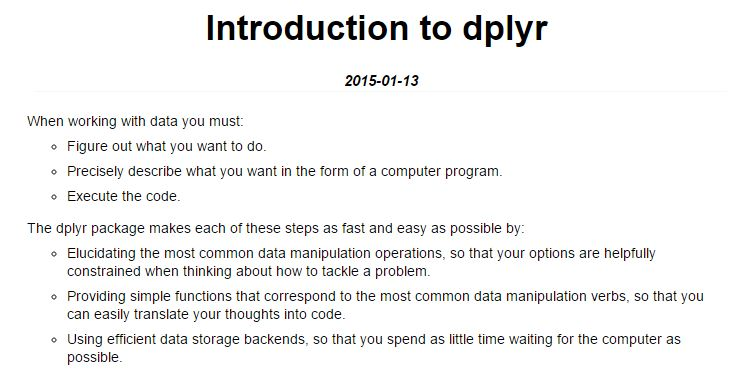
\includegraphics[width=1.1\linewidth]{images/introdplyr}

\end{figure}



<p>====
[fragile]
\frametitle{Installing dplyr}
Straightforward \texttt{R} package installation.

\begin{verbatim}
install.packages("dplyr")
library(dplyr)

# Data Set Examples
# 1. iris
# 2. mtcars

\end{verbatim}


%=== %

[fragile]
\frametitle{iris data set}

\begin{verbatim}
> names(iris)
[1] "Sepal.Length"
[2] "Sepal.Width" 
[3] "Petal.Length"
[4] "Petal.Width" 
[5] "Species"    
\end{verbatim}


<p>====== %

[fragile]
\frametitle{mtcars data set}
\begin{verbatim}
> names(mtcars)
[1] "mpg"  "cyl"  "disp" "hp"  
[5] "drat" "wt"   "qsec" "vs"  
[9] "am"   "gear" "carb"
\end{verbatim}

<p>
[fragile]
\frametitle{Example Data Sets}
\begin{verbatim}
dim(iris)
class(iris)
mode(iris)

dim(mtcars)
class(mtcars)
mode(mtcars)
\end{verbatim}

<p>=== %

\frametitle{dplyr; Single Table Verbs}
dplyr aims to provide a function for each basic verb of data manipulating:

* \texttt{ filter() } (and \texttt{  slice() })
* \texttt{ arrange() }
* \texttt{ select() } (and \texttt{  rename() })
* \texttt{ distinct() }
* \texttt{ mutate() } (and \texttt{  transmute() })
* \texttt{ summarise() }
* \texttt{ sample\_n() } and \texttt{  sample\_frac() }
\end{itemize}
%\begin{figure}
%\centering
%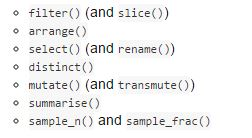
\includegraphics[width=0.7\linewidth]{images/singletableverbs}
%
%\end{figure}


%== %
[fragile]

\frametitle{The \texttt{glimpse()}} 

* dplyr also provides a function \texttt{glimpse()} that makes it easy to look at our data in a transposed view. 

* It's similar to the \texttt{str()} (structure) function, but has a few advantages (see \texttt{?glimpse}).

\end{itemize}

%== %
[fragile]

\frametitle{The \texttt{glimpse()} }
\begin{figure}
\centering
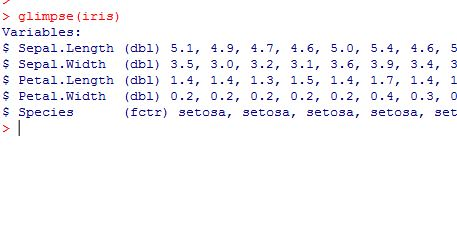
\includegraphics[width=1.2\linewidth]{images/irisglimpse}

\end{figure}


%== %
[fragile]
\frametitle{The \texttt{glimpse()} }

\begin{figure}
\centering
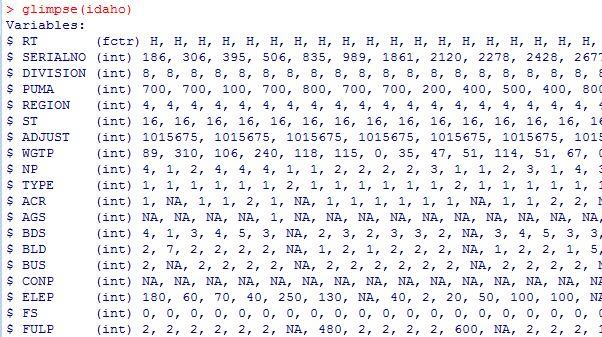
\includegraphics[width=1.2\linewidth]{images/idahoglimpse}

\end{figure}


%== %
[fragile]
\frametitle{ Multiple Selections with \texttt{select()} }

\begin{verbatim}
idaho2 = select(idaho,
num_range("idaho",1:6),
contains("AX"),
starts_with("FK"),
starts_with("SM"),
ends_with("SP") 
)
\end{verbatim}



%== %
[fragile]
\frametitle{ Dropping Variables with \texttt{select()} }

\begin{verbatim}

# Drop variables
select(iris, -starts_with("Petal"))
select(iris, -ends_with("Width"))
select(iris, -contains("etal"))
select(iris, -matches(".t."))
select(iris, -Petal.Length, -Petal.Width)
\end{verbatim}




%=== %

\frametitle{Grouped operations}


* The verbs are useful, but they become really powerful when you combine them with the idea of “group by”, repeating the operation individually on groups of observations within the dataset. 
* In dplyr, you use the \texttt{group\_by()} function to describe how to break a dataset down into groups of rows. 
* You can then use the resulting object in exactly the same functions as above; they’ll automatically work “by group” when the input is a grouped.
\end{itemize}



<p>===
\frametitle{\texttt{group\_by }}

Group a tbl by one or more variables.\\ <p>

\textbf{Description}\\ <p>

Most data operations are useful done on groups defined by variables in the the dataset. The
\textbf{group\_by} function takes an existing tbl and converts it into a grouped tbl where operations are
performed "by group".


<p> %

\frametitle{Summary Statistics}
You use \texttt{summarise()} with aggregate functions, which take a vector of values, and return a single number.\\ <p> There are many useful functions in base R like \texttt{min()}, \texttt{max()}, \texttt{mean()}, \texttt{sum()}, \texttt{sd()}, \texttt{median()}, and \texttt{IQR()}.\\ <p> dplyr provides a handful of others:

* 
\texttt{n()}: number of observations in the current group
* 
\texttt{n\_distinct(x)}: count the number of unique values in x.
\end{itemize}

%
%first(x), last(x) and nth(x, n) - these work similarly to x[1], x[length(x)], and x[n] but give you more control of the result if the value isn’t present.

<p>======
[fragile]
\frametitle{Grouping with the \texttt{group\_by} command}
\begin{verbatim}

iris.sp <- group_by(iris,Species)
class(iris.sp)

summarise(iris.sp,mean(Sepal.Length), sd(Petal.Length))

\end{verbatim}

%== %

\begin{figure}
\centering
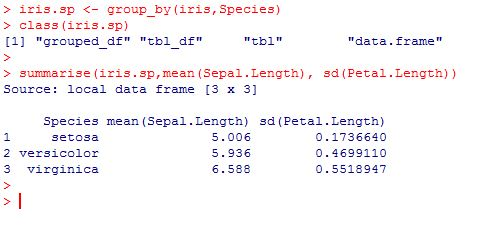
\includegraphics[width=1.05\linewidth]{images/irisgroupby}
\end{figure}


%= %

\begin{figure}
\centering
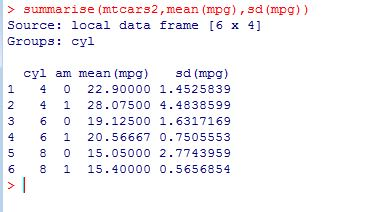
\includegraphics[width=1.1\linewidth]{images/mtcarssummarise}
\label{fig:mtcarssummarise}
\end{figure}



<p>======

\frametitle{Filter rows with \texttt{filter()}}

* \texttt{filter()} allows you to select a subset of the rows of a data frame. 
* The first argument is the name of the data frame, and the second and subsequent are filtering expressions evaluated in the context of that data frame.
\end{itemize}




<p>======
[fragile]

\begin{verbatim}
iris.vir1 <- filter(iris,Species=="virginica")

# Species is Virginica OR Petal.length is 
# greater than 3.2

iris.vir2 <- filter(iris,
Species=="virginica" | Petal.Length >3.2)

iris.vir3 <- filter(iris,
Species=="virginica" & Petal.Length >3.9)

\end{verbatim}


<p>=====

\frametitle{Ordering Data Sets with \texttt{arrange()}}

* \texttt{arrange()} works similarly to \texttt{filter()} except that instead of filtering or selecting rows, it reorders them. 

* It takes a data frame, and a set of column names (or more complicated expressions) to order by.

* If you provide more than one column name, each additional column will be used to break ties in the values of preceding columns.

* Use \texttt{desc()} (or \texttt{rev()}) to order a column in descending order.

%arrange(flights, desc(arr_delay))
\end{itemize}

<p>==== %

\begin{figure}
\centering
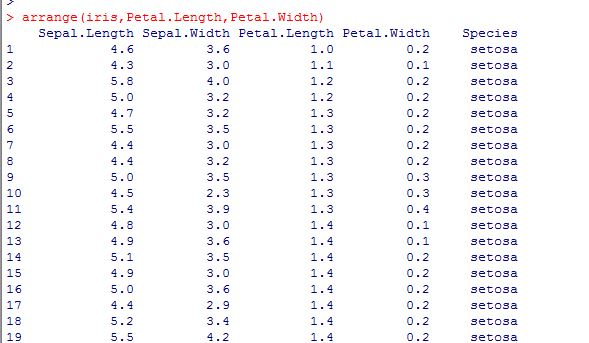
\includegraphics[width=0.97\linewidth]{images/irisarrange}

\end{figure}



<p>=== %


\begin{figure}
\centering
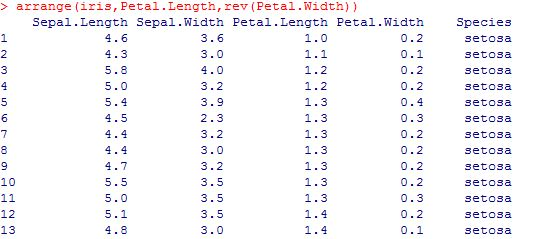
\includegraphics[width=0.97\linewidth]{images/irisarrange2}

\end{figure}



% Graphics: irisarrange

<p>==

\frametitle{Select columns with \texttt{select()}}

* Often you work with large datasets with many columns where only a few are actually of interest to you. 
* select() allows you to rapidly zoom in on a useful subset using operations that usually only work on numeric variable positions.
\end{itemize}



\frametitle{Selection Options with \texttt{select()}}
\begin{figure}
\centering
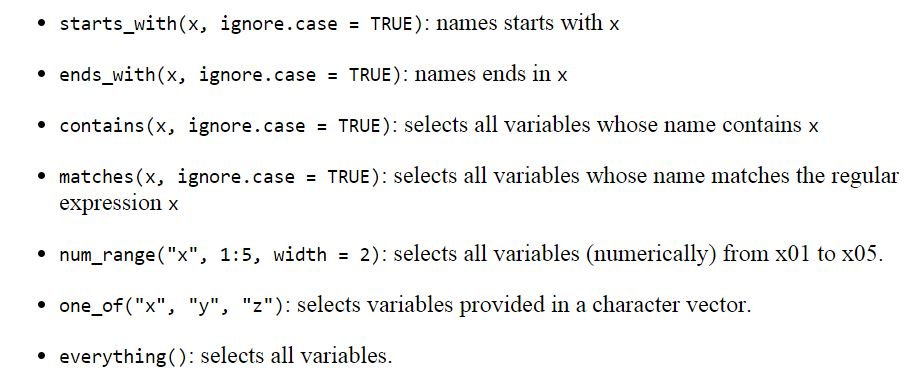
\includegraphics[width=01.05\linewidth]{images/selectoptions}
\end{figure}



\frametitle{Selection Options with \texttt{select()}}

\begin{figure}
\centering
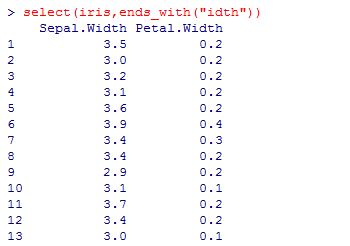
\includegraphics[width=0.69\linewidth]{images/selectendswith}
\end{figure}





\frametitle{Selection Options with \texttt{select()}}

\begin{figure}
\centering
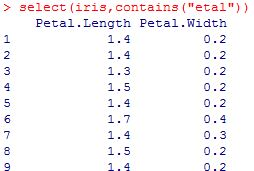
\includegraphics[width=0.69\linewidth]{images/selectioncontaints}
\end{figure}





\frametitle{Sampling rows with \texttt{sample\_n()} and \texttt{sample\_frac()}}

* You can use \texttt{sample\_n()} and \texttt{sample\_frac()} to take a random sample of rows, either a fixed number for \texttt{sample\_n()} or a fixed fraction for \texttt{sample\_frac()}.
\end{itemize}



\frametitle{Sampling rows with \texttt{sample\_n()} and \texttt{sample\_frac()}}

\begin{figure}
\centering
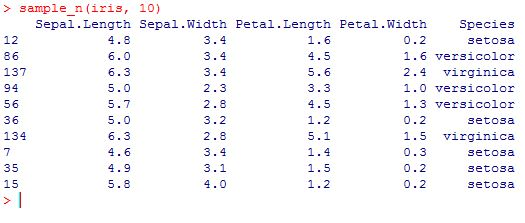
\includegraphics[width=1.07\linewidth]{images/irissample1}
\end{figure}


%------------------------------------------------------------------------------------ %

\frametitle{Sampling rows with \texttt{sample\_n()} and \texttt{sample\_frac()}}

\begin{figure}
\centering
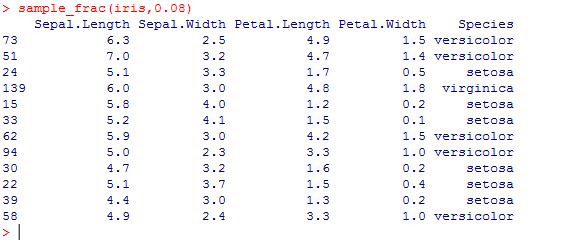
\includegraphics[width=1.07\linewidth]{images/irissample2}
\end{figure}


%------------------------------------------------------------------------------------ %

\frametitle{Sampling rows with \texttt{sample\_n()} and \texttt{sample\_frac()}}

\begin{figure}
\centering
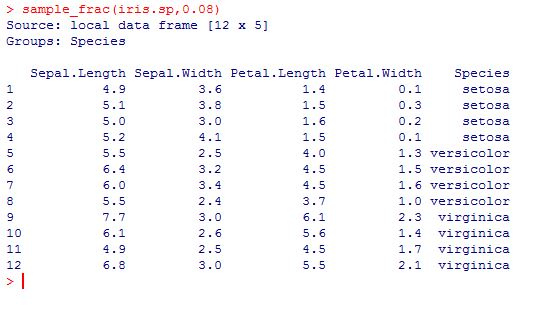
\includegraphics[width=1.07\linewidth]{images/irissample3}
\end{figure}


<p>====
[fragile]
\frametitle{Add new columns with \texttt{mutate()} }

As well as selecting from the set of existing columns, it’s often useful to add new columns that are functions of existing columns. This is the job of \texttt{mutate()}:


\begin{verbatim}
iris2 =  mutate(iris, 
PW2 = log(Petal.Width), 
PL2=sqrt(Petal.Length) )

head(iris2)
\end{verbatim}


<p> %
%% Graph irismutate


\frametitle{Add new columns with \texttt{mutate()} }
\begin{figure}
\centering
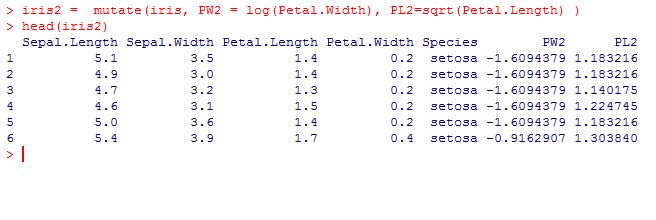
\includegraphics[width=1.2\linewidth]{images/irismutate}

\end{figure}


<p>==
[fragile]

\frametitle{Add new columns with \texttt{mutate()} }
\texttt{mutate} allows you to refer to columns that you just created:

\begin{verbatim}
iris3 =  mutate(iris, 
PW2 = log(Petal.Width), 
PL2=sqrt(Petal.Length), 
Ratio=PL2/PW2 )

head(iris3)
\end{verbatim}
 
% %


\frametitle{Add new columns with \texttt{mutate()} }
\begin{figure}
\centering
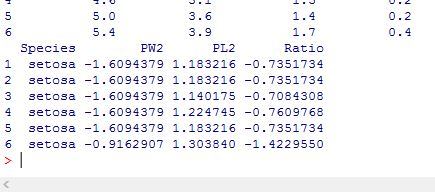
\includegraphics[width=0.9\linewidth]{images/irismutate2}

\end{figure}




%% Graphic irismutate2

\frametitle{Multiple table verbs}

As well as verbs that work on a single \texttt{tbl}, there are also a set of useful verbs that work with two \texttt{tbl}s at a time: joins and set operations.


\frametitle{Joins}
dplyr implements the four most useful joins from SQL:


* \texttt{inner\_join(x, y)}: matching x + y
* \texttt{left\_join(x, y)}: all x + matching y
* \texttt{semi\_join(x, y)}: all x with match in y
* \texttt{anti\_join(x, y)}: all x without match in y
\end{itemize}


\begin{figure}
\centering
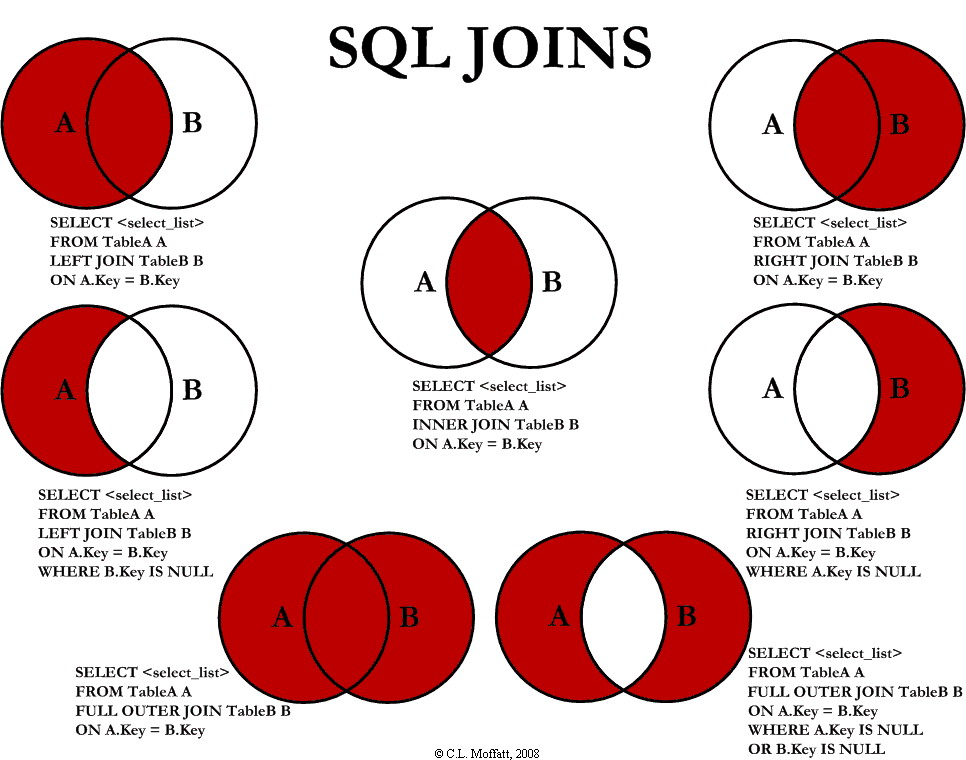
\includegraphics[width=1.00\linewidth]{images/SQLjoins}

\end{figure}



\frametitle{Joins}
Pretend data set listing country of origin for each species.
The variables ``Species" is common to both data frames.
\begin{figure}
\centering
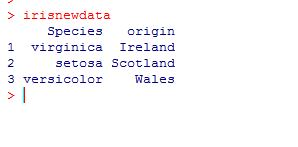
\includegraphics[width=0.7\linewidth]{images/irisnewdata}
\caption{Second Data Frame}
\label{fig:irisnewdata}
\end{figure}




\frametitle{Joins}
\begin{figure}
\centering
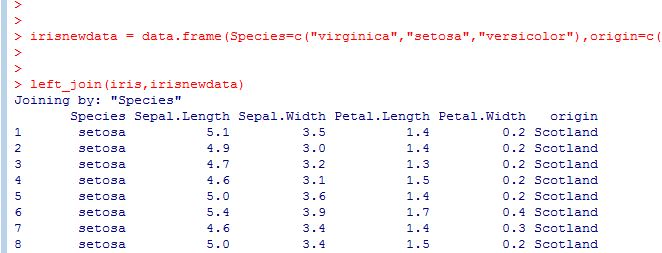
\includegraphics[width=0.97\linewidth]{images/irisjoin}

\label{fig:irisjoin}
\end{figure}


<p>= %


\frametitle{Set Theory Operations}

dplyr implements the methods for set theory operations


* \texttt{intersect(x, y)}: all rows in both x and y
* \texttt{union(x, y)}: rows in either x or y
* \texttt{setdiff(x, y)}: rows in x, but not y
\end{itemize}



<p>
